% SPDX-License-Identifier: Apache-2.0
% Copyright 2026 Hakan Damar and Theseus Guard, Inc.
% Licensed under the Apache License, Version 2.0 (http://www.apache.org/licenses/LICENSE-2.0)
% Developed by Theseus Guard Research (https://www.theseusguard.com)
% Repository: https://github.com/Theseus-Guard/ZTCP
% Contact: TG-Team <contact@theseusguard.com> | https://www.theseusguard.com/contact
% ArXiv / MLSys / SOSP Preprint Manuscript
\documentclass[10pt,twocolumn]{article}

\usepackage[utf8]{inputenc}
\usepackage[T1]{fontenc}
\usepackage[margin=0.78in]{geometry}
\usepackage{amsmath,amssymb,amsfonts,amsthm}
\usepackage{booktabs}
\usepackage{multirow}
\usepackage{hyperref}
\usepackage{url}
\usepackage{xcolor}
\usepackage{tikz}
\usepackage{pgfplots}
\pgfplotsset{compat=1.18}

\hypersetup{
    colorlinks=true,
    linkcolor=blue!60!black,
    citecolor=blue!60!black,
    urlcolor=blue!60!black
}

\newtheorem{theorem}{Theorem}
\newtheorem{corollary}{Corollary}

\title{\Large \textbf{Zero-Trust Cold Pages: Accelerating Distributed RDMA KV-Cache Offloading via Fused Asymmetric Quantization and Authenticated Encryption}}

\author{
    \textbf{Hakan Damar} \\
    Theseus Guard, Inc. \\
    \texttt{hakan.damar@theseusguard.com} \\
    \small\url{https://github.com/Theseus-Guard/ZTCP} $\cdot$ \textbf{DOI:} \href{https://doi.org/10.5281/zenodo.23555749}{\texttt{10.5281/zenodo.23555749}}
}

\date{October 2026}

\begin{document}
\maketitle

\begin{abstract}
Disaggregated Large Language Model (LLM) serving and hierarchical Key-Value (KV) cache pooling over RDMA (e.g., Mooncake, LMCache, SGLang HiCache, NVIDIA NIXL) mitigate GPU HBM capacity limits by offloading evicted KV pages to distributed DRAM and NVMe tiers. However, current distributed KV-cache architectures suffer from a dual bottleneck: (1) \textbf{bandwidth bloat}, where evicted KV pages traverse PCIe and RDMA fabrics in their uncompressed runtime precision (\texttt{BF16}/\texttt{FP16}/\texttt{FP8}) or incur costly host-side temporary buffer copies during serialization, and (2) \textbf{plaintext exposure and cross-tenant contamination}, where sensitive activation vectors leave the compute node unencrypted and vulnerable to prompt-inversion recovery, cross-request cache mixing, or remote memory poisoning.

We present \textbf{Zero-Trust Cold Pages (ZTCP)}, a storage- and transport-boundary architecture developed at \textbf{Theseus Guard} that extends the \textbf{Zero-Trust AI Data Plane (ZT-ADP)}, the \textbf{L1 Precedent Decision Cache}, and the \textbf{DREP (\textit{Detect--Route--Enforce--Prove})} governance lifecycle~\cite{theseusguard2026patent} to distributed RDMA KV-cache pools. ZTCP combines \textbf{RoPE-preserving asymmetric cold-page quantization} with \textbf{256-bit IETF RFC 8439 ChaCha20 stream encryption and 128-bit SipHash-2-4-128 Encrypt-then-MAC authentication} (distinct from ChaCha20-Poly1305) over the full 32-byte Associated Data (AAD) header and ordered ciphertext payload. By keeping active GPU Attention KV in its native hot precision while compressing cold pages by \textbf{2.67$\times$--2.94$\times$} prior to encryption, ZTCP reduces cryptographic work by over 62\%. Across $N=5$ independent OS process runs ($\times 50$ batch iterations per run) on an Apple M3 Max CPU (\texttt{Qwen/Qwen3.6-35B-A3B} GQA page geometry), our C++17 ARMv8.5-A FP16 NEON implementation achieves \textbf{2.35 $\pm$ 0.01 GB/s} single-core hot-byte egress throughput (\textbf{20.85$\times$} vs.\ multi-operator Python/PyTorch), \textbf{17.47 $\pm$ 0.43 GB/s} (\textbf{6.55 $\pm$ 0.16 GB/s} wire) allocated 64-page batch egress (\textbf{23.02 $\pm$ 0.38 GB/s} hot ingress), and \textbf{26.65 $\pm$ 0.46 GB/s} hot-byte (\textbf{10.00 $\pm$ 0.17 GB/s} wire) 256-page preallocated CPU buffer peak egress (\textbf{25.84 $\pm$ 0.28 GB/s} hot peak ingress; \textbf{236.05$\times$} descriptive tier ratio over Python and \textbf{11.32$\times$} over single-core C++). In an analytical serial-egress 100GbE RoCEv2 model ($11.2\text{ GB/s}$ effective goodput), our measured CPU throughput exceeds the Theorem~1 serial break-even threshold ($17.93\text{ GB/s}$ hot / $6.73\text{ GB/s}$ wire) by 48.6\%, reducing modeled 4,096-token prefix transfer latency across 64 layers ($1,073.74\text{ MB}$ SI / $1,024.0\text{ MiB}$) from \textbf{95.87 ms} (unencrypted raw \texttt{BF16}) to \textbf{76.28 $\pm$ 0.70 ms} (\textbf{1.26 $\pm$ 0.01$\times$} speedup), while projecting \textbf{37.10 ms} (\textbf{2.58$\times$}) under hypothetical GPU SRAM execution ($950\text{ GB/s}$).
\end{abstract}

\section{Introduction}
Long-context reasoning, multi-turn agentic workflows, and prefill-decode (PD) disaggregation rely heavily on reusing cached Key-Value (KV) states across requests~\cite{kwon2023vllm,zheng2024sglang,qin2024mooncake}. Because high-bandwidth GPU memory (HBM) is scarce and costly, production inference engines increasingly adopt three-tier hierarchical KV caching (which we denote as Memory Tiers M1--M3 to distinguish them from the L1--L3 AI governance evaluation layers):
\begin{itemize}
    \item \textbf{Tier M1 (Hot GPU HBM):} Active GPU memory executing Attention kernels in runtime precision (\texttt{BF16}, \texttt{FP16}, or \texttt{FP8}).
    \item \textbf{Tier M2 (Warm Host Memory):} Node-local pinned Host DRAM or NVMe SSD.
    \item \textbf{Tier M3 (Cold Distributed Pool):} Cross-node RDMA memory pools such as Mooncake Store~\cite{qin2024mooncake}, LMCache Multiprocess (MP) mode~\cite{cheng2025lmcache,liu2024cachegen}, or 3FS.
\end{itemize}

\subsection{Architectural Gaps in Production Systems}
Recently, NVIDIA TensorRT-LLM introduced \textit{NVFP4 Cold-Page Compression}~\cite{nvidia2026trtllmcoldpage} for worker-local Host and Disk tiers, demonstrating that KV pages can be compressed strictly at the cold storage boundary without altering active GPU Attention precision, page identity, or block reuse scheduling. However, our audit of production distributed inference stacks reveals three critical architectural gaps when cold pages cross node boundaries over RDMA:

\begin{enumerate}
    \item \textbf{Locality Limit in TensorRT-LLM:} TensorRT-LLM's cold-page codec operates exclusively on the worker-local \texttt{GPU $\leftrightarrow$ Host/Disk} path; inter-node disaggregated transfers over NIXL transmit the uncompressed hot KV representation~\cite{nvidia2026trtllmcoldpage}.
    \item \textbf{Uncompressed RDMA Transport in SGLang HiCache \& Mooncake:} In SGLang's \texttt{HiCacheStorage} and \texttt{MooncakeHostTensorAllocator}, host staging buffers are allocated at the exact element byte size of the hot GPU tensor. Offloading a 4,096-token prefix across 64 layers (GQA-8, \texttt{head\_dim=128}, \texttt{BF16}) transmits \textbf{1,073.74 MB} ($1,024.0\text{ MiB}$) of raw bytes across the RDMA fabric.
    \item \textbf{Host Double-Buffering \& Plaintext Leakage in LMCache:} While LMCache MP mode~\cite{cheng2025lmcache} provides \texttt{SerdeL2AdapterWrapper} for L2 quantization (\texttt{fp8}, \texttt{turboquant}) and encryption (\texttt{aesgcm}), every store/load batch invokes \texttt{L1Manager.reserve\_write(temp\_keys)} to allocate secondary host buffers and executes quantization and CPU AES-GCM as discrete memory-bound passes. Moreover, LMCache's built-in \texttt{aesgcm} derives keys from a single fleet-wide master secret rather than per-tenant ephemeral sessions, leaving multi-tenant pools exposed to cross-request KV contamination (e.g., LMCache Issue \#4385) and insider inspection.
\end{enumerate}

\subsection{Contributions \& Scope Separation}
This paper makes four contributions while explicitly separating what is \textbf{empirically measured in our open-source CPU artifact} from \textbf{target production/enterprise hardware extensions}:
\begin{enumerate}
    \item \textbf{Formal Compress-then-Encrypt Break-Even vs.\ Wire-Saturation Model:} We prove that when cold-page compression ($r > 1$) is combined with authenticated encryption, serial transfer achieves net latency reduction over unencrypted raw transfer whenever hot-byte processing throughput exceeds the \textit{break-even bound} $BW_{\text{fused,hot}} > \frac{r}{r-1} BW_{\text{net}}$, whereas full line-rate \textit{wire saturation} requires $BW_{\text{fused,wire}} \ge BW_{\text{net}} \iff BW_{\text{fused,hot}} \ge r \cdot BW_{\text{net}}$.
    \item \textbf{RoPE-Preserving Asymmetric Cold-Page Wire Format:} We design a 64-byte-aligned cold-page format (\texttt{32B AAD Header + Encrypted Payload + 16B MAC}) supporting both GQA (\texttt{Qwen/Qwen3.6-35B-A3B} profile) and single-buffer DeepSeek Multi-head Latent Attention (MLA, \texttt{DeepSeek-V4.1-Flash} profile)~\cite{deepseek2024v3}. On synthetic RoPE-outlier KV pages (\texttt{seed=42}), preserving the 64-element RoPE sub-vector in 8-bit (\texttt{PRESERVE\_FP8}) while quantizing NoPE and Value buffers to 4-bit yields \textbf{2.67$\times$} compression with \textbf{0.9961--0.9962} simulated single-page \textit{Attention Output Cosine Similarity} on GQA and \textbf{2.94$\times$} compression with \textbf{0.9995} \textit{Softmax Attention Weights Cosine Similarity} on single-buffer MLA (where $V=\text{None}$).
    \item \textbf{Verified C++17 ARMv8.5-A FP16 NEON Codec (RFC 8439 ChaCha20 + SipHash-2-4-128):} We implement a unified C++17 SIMD codec that quantizes 32--64 FP16 values per vector pass (\texttt{vmaxvq\_f16} group abs-max, vectorized \texttt{vdivq\_f32} / scalar \texttt{FP32} reciprocal division narrowed to \texttt{FP16}, and vectorized \texttt{vmulq\_f16} + \texttt{vcvtnq\_s16\_f16} nearest-even rounding), encrypts all quantized sub-vectors, per-group FP16 scales, and padding with 256-bit IETF RFC 8439 ChaCha20 (4-block transposed NEON), and authenticates the 32B header and ordered ciphertext via 128-bit SipHash-2-4-128. Across $N=5$ independent process runs on Apple M3 Max, the codec achieves \textbf{26.65 $\pm$ 0.46 GB/s} hot-byte (\textbf{10.00 $\pm$ 0.17 GB/s} wire) peak egress and \textbf{25.84 $\pm$ 0.28 GB/s} hot-byte peak ingress into preallocated CPU buffers.
    \item \textbf{Transactional Session Keyring, Zero-Fork Upstream Hooks \& DREP Governance Integration:} We provide zero-copy plugin ABIs for SGLang HiCache, LMCache, and Mooncake, backed by a thread-safe, generation-bound \texttt{EphemeralSessionKeyRing} that uses HMAC-SHA256-based domain-separated per-generation key derivation and enforces atomic pre-encryption nonce reservation, monotonic per-slot freshness watermarks, and CSPRNG-salted in-process crypto-shredding, alongside architectural integration with the \textbf{Theseus Guard DREP} control plane~\cite{theseusguard2026patent,theseusguard2026g1}.
\end{enumerate}

\section{Threat Model \& Break-Even Theorem}

\subsection{Zero-Trust Distributed KV Threat Model}
We consider a multi-tenant LLM serving cluster where compute nodes offload cold KV pages across shared host DRAM, PCIe switches, RoCEv2/InfiniBand fabrics, and remote Mooncake storage servers that are treated as \textbf{untrusted}. (In enterprise deployments, compute nodes additionally operate inside hardware-enforced Trusted Execution Environments such as NVIDIA H100/B200 Confidential Computing with Intel TDX or AMD SEV-SNP host enclaves; our public artifact evaluates the cryptographic codec and session state machine in user-space CPU memory.) An adversary or faulty storage controller may:
\begin{itemize}
    \item \textbf{Passively eavesdrop (Prompt Inversion):} Read evicted KV pages or unencrypted scale factors in remote DRAM/SSD to reconstruct user prompts and confidential enterprise documents.
    \item \textbf{Cross-Tenant Contamination:} Return Tenant A's cached KV page to Tenant B due to hash collisions or indexing bugs.
    \item \textbf{Active KV Poisoning, Scale/Block Splicing \& Stale Replay:} Flip bits in remote KV blobs, swap 16-byte quantized blocks, tamper with FP16 group scales, or replay an older superseded KV page version for a given token slot.
    \item \textbf{Long-Term Ciphertext Archival \& Multi-Compartment Contagion:} In sovereign defense and multi-agency HPC environments~\cite{damar2023hybrid}, adversaries archive intercepted traffic or exploit shared cache pools. ZTCP employs full 256-bit RFC 8439 ChaCha20 session keys (derived via HMAC-SHA256-based domain-separated per-generation derivation mixed with a per-session 256-bit CSPRNG secret) and strict per-page 32-byte AAD binding; enterprise control planes can additionally pair session establishment with NIST \textbf{FIPS 203 ML-KEM} and \textbf{FIPS 204 ML-DSA}~\cite{nist2024pqc}.
\end{itemize}

\subsection{Break-Even Bound vs.\ Link Wire-Saturation Bound}
Standard confidential computing encrypts uncompressed tensors ($r=1$), inevitably adding latency. ZTCP compresses the cold page by factor $r = B_{\text{hot}} / B_{\text{cold}} > 1$ \textit{first} and encrypts/authenticates only the reduced $B_{\text{cold}}$ bytes. Crucially, one must distinguish between the \textbf{hot-byte processing throughput} $BW_{\text{fused,hot}} = B_{\text{hot}} / t_{\text{page}}$ and the \textbf{encoded wire output throughput} $BW_{\text{fused,wire}} = B_{\text{cold}} / t_{\text{page}} = BW_{\text{fused,hot}} / r$.

\begin{theorem}[Serial Compress-then-Encrypt Break-Even Bound]
Let $B_{\text{hot}}$ be the byte size of a hot KV page, $r = B_{\text{hot}} / B_{\text{cold}} > 1$ be the net cold-page compression ratio (including the 32B AAD header and 16B MAC tag), $BW_{\text{net}}$ be the effective RDMA network goodput, and $BW_{\text{fused,hot}}$ be the fused kernel throughput measured in hot KV bytes processed per second (all in consistent SI units, $1\text{ GB/s} = 10^9\text{ B/s}$). In a non-overlapped serial pipeline (compute followed by wire transfer), the total transfer latency of an authenticated, encrypted ZTCP cold page ($T_{\text{ztcp}}$) is strictly smaller than that of an unencrypted raw KV page ($T_{\text{raw}}$) if and only if:
{\small
\begin{equation}
    BW_{\text{fused,hot}} > \tfrac{r}{r - 1} BW_{\text{net}}
    \iff BW_{\text{fused,wire}} > \tfrac{1}{r - 1} BW_{\text{net}}
    \label{eq:breakeven}
\end{equation}
}
\end{theorem}

\begin{proof}
Transmitting an unencrypted raw KV page over RDMA requires $T_{\text{raw}} = \frac{B_{\text{hot}}}{BW_{\text{net}}}$. In serial ZTCP execution, the page undergoes fused quantization + AEAD in time $\frac{B_{\text{hot}}}{BW_{\text{fused,hot}}}$ followed by RDMA transmission of $B_{\text{cold}} = \frac{B_{\text{hot}}}{r}$ bytes in time $\frac{B_{\text{hot}}}{r \cdot BW_{\text{net}}}$. Requiring $T_{\text{ztcp}} < T_{\text{raw}}$ yields:
{\footnotesize
\begin{equation*}
    \tfrac{B_{\text{hot}}}{BW_{\text{fused,hot}}} + \tfrac{B_{\text{hot}}}{r \cdot BW_{\text{net}}} < \tfrac{B_{\text{hot}}}{BW_{\text{net}}}
    \iff \tfrac{1}{BW_{\text{fused,hot}}} < \tfrac{r - 1}{r \cdot BW_{\text{net}}}
\end{equation*}
}
Inverting both sides establishes Inequality~\eqref{eq:breakeven}, with net serial speedup $S = \left(\frac{1}{r} + \frac{BW_{\text{net}}}{BW_{\text{fused,hot}}}\right)^{-1}$.
\end{proof}

\textbf{Corollary 1 (Break-Even vs.\ Full Link Wire Saturation):} Whereas break-even requires $BW_{\text{fused,hot}} > \frac{r}{r-1} BW_{\text{net}}$, keeping an RDMA link 100\% saturated with compressed cold blobs requires $BW_{\text{fused,wire}} \ge BW_{\text{net}} \iff BW_{\text{fused,hot}} \ge r \cdot BW_{\text{net}}$. For GQA cold pages with \texttt{INT4\_SYM + Preserve RoPE (FP8)} ($r = 262,144 / 98,352 = 2.6654$, $\frac{r}{r-1} = 1.6005$):
\begin{itemize}
    \item \textbf{100GbE RoCEv2 ($BW_{\text{net}} = 11.2\text{ GB/s}$):} Serial break-even requires $BW_{\text{fused,hot}} > \mathbf{17.93\text{ GB/s}}$ ($6.73\text{ GB/s}$ wire), while 100\% wire saturation requires $BW_{\text{fused,hot}} \ge \mathbf{29.85\text{ GB/s}}$ ($11.20\text{ GB/s}$ wire). Our measured M3 Max CPU peak throughput (\textbf{26.65 $\pm$ 0.46 GB/s} hot / \textbf{10.00 $\pm$ 0.17 GB/s} wire on \texttt{INT4\_SYM}, and \textbf{23.76 $\pm$ 0.27 GB/s} hot / \textbf{10.40 $\pm$ 0.12 GB/s} wire on \texttt{K8V4\_ASYM}, exceeding its $19.92\text{ GB/s}$ hot break-even bound by 19.3\%) exceeds the \texttt{INT4\_SYM} 100GbE break-even bound by 48.6\% (corresponding to an analytical ratio $BW_{\text{fused,wire}} / BW_{\text{net}}$ of 89.3\%--92.9\% of modeled 100GbE wire capacity from a single CPU socket---not a live NIC measurement---and yielding a $1.26 \pm 0.01\times$ analytical serial speedup over unencrypted raw \texttt{BF16}).
    \item \textbf{400GbE NDR InfiniBand ($BW_{\text{net}} = 45.0\text{ GB/s}$):} Break-even requires $BW_{\text{fused,hot}} > \mathbf{72.02\text{ GB/s}}$ ($27.02\text{ GB/s}$ wire) and full wire saturation requires $BW_{\text{fused,hot}} \ge \mathbf{119.94\text{ GB/s}}$ ($45.00\text{ GB/s}$ wire), which exceeds single-socket CPU throughput and motivates GPU SRAM execution.
\end{itemize}

\section{ZTCP Architecture \& Cryptographic Construction}

\subsection{Compact Cold-Page Wire Specification \& Bijective Nonce}
Each cold KV page is encoded as a contiguous, 64-byte DMA-aligned binary blob:
\begin{enumerate}
    \item \textbf{32-Byte Plaintext Authenticated Header (AAD):}
    {\footnotesize
    \begin{verbatim}
struct ColdPageHeaderRaw {
  uint16_t magic;          // 0x5A54 ("ZT")
  uint8_t  version;        // 1
  uint8_t  flags;          // Preset | RoPE
  uint32_t tenant_id_hash; // BLAKE2s-32
  uint32_t model_id_hash;  // Model/Snapshot
  uint16_t layer_id;       // Layer index
  uint16_t head_group_id;  // Group index
  uint64_t page_token_hash;// BLAKE2s-64
  uint64_t sequence_nonce; // Monotonic u64
}; // 32 bytes exact
    \end{verbatim}
    }
    \item \textbf{Bijective 96-Bit ChaCha20 Nonce Packing:} Rather than XOR-mixing header fields (which would allow cross-field XOR cancellations between \texttt{sequence\_nonce} and \texttt{model\_id\_hash}/\texttt{page\_token\_hash}), ZTCP packs the 96-bit (12-byte) IETF RFC 8439 ChaCha20 nonce bijectively as:
    {\footnotesize
    \begin{equation*}
        \texttt{nonce}_{96} = \texttt{seq\_nonce}_{64} \;\|\; \texttt{layer\_id}_{16} \;\|\; \texttt{head\_group\_id}_{16}
    \end{equation*}
    }
    \item \textbf{Encrypted Quantized Payload \& Scales:} Contains the separated Key RoPE slice (\texttt{PRESERVE\_FP8}: 1B INT8 data + 2B FP16 scale per 16 elements), Key NoPE slice (packed 4-bit nibbles or 8-bit data + 2B FP16 scale per 16 elements), Value slice (packed 4-bit nibbles or 8-bit data + 2B FP16 scale per 16 elements; omitted for single-buffer DeepSeek-MLA), and deterministic zero tail padding to a 64-byte boundary. \textbf{All sections---including all FP16 scale arrays and tail padding---are encrypted under the 256-bit RFC 8439 ChaCha20 keystream.}
    \item \textbf{16-Byte Authentication Tag (Encrypt-then-MAC):} Computed sequentially via standard \textbf{SipHash-2-4-128} (Aumasson--Bernstein, using two 64-bit MAC keys $mk_0, mk_1$ derived via domain-separated HMAC-SHA256) over the exact byte sequence $\texttt{header\_32b} \;\|\; \texttt{ordered\_ciphertext\_payload}$.
\end{enumerate}

\subsection{Unified Single/Batch/Peak Execution \& L1 Scale Staging}
All three native C++17 entrypoints (\texttt{fused\_encode\_cold\_page\_cpu}, \texttt{fused\_encode\_cold\_pages\_batch\_cpu}, and \texttt{fused\_encode\_cold\_pages\_peak\_into\_cpu}) invoke the same canonical single-page encoder (\texttt{encode\_one\_cold\_page\_into\_cpu}), guaranteeing bit-for-bit identical wire output (\texttt{single == batch == peak}):
\begin{enumerate}
    \item \textbf{Multi-Group FP16 Vector Quantization (32--64 Elements):} On ARMv8.5-A NEON (\texttt{csrc/fused\_cold\_page\_cpu.cpp}), 128-bit registers load 32 or 64 contiguous \texttt{FP16} values (two or four 16-element groups) and compute group abs-maxima via \texttt{vmaxvq\_f16}. Each maximum is widened to \texttt{FP32} (\texttt{float}) to compute the group scale (\texttt{fmax * (1.0f / 7.0f)} or \texttt{1.0f / 127.0f}, stored as \texttt{FP16}) and its exact IEEE-754 \texttt{FP32} reciprocal (vectorized \texttt{vdivq\_f32} in 4-group kernels; scalar \texttt{1.0f / static\_cast<float>(sc)} in 2-group fallback), which is narrowed back to \texttt{FP16} (\texttt{vcvt\_f16\_f32} / \texttt{vdupq\_n\_f16}) for vectorized \texttt{FP16} multiplication (\texttt{vmulq\_f16}), round-to-nearest-even (\texttt{vcvtnq\_s16\_f16}), and nibble packing (\texttt{vuzpq\_u8}, \texttt{vorrq\_u8}) into 128-bit registers.
    \item \textbf{In-Register ChaCha20 Encryption \& SipHash-2-4-128 Absorption:} A 4-block transposed NEON engine (\texttt{chacha20\_4blocks\_rfc8439}) generates 256 bytes of RFC 8439 ChaCha20 keystream per refill using all 256 bits ($k_0, k_1, k_2, k_3$) of the session encryption key. For quantized vectors (\texttt{q\_rope}, \texttt{q\_nope}, \texttt{q\_v}, which form \textbf{83.3\%} of a GQA \texttt{INT4\_SYM} page), 16B/32B/64B register groups are XOR-encrypted and absorbed into the streaming SipHash-2-4-128 state prior to a single store to the output buffer (falling back to a byte-exact scalar path whenever a partial MAC word is pending or the keystream cursor is unaligned).
    \item \textbf{L1 Stack-Resident Scale Staging:} Because the wire layout places each section's contiguous \texttt{FP16} scale array (\texttt{s\_rope}, \texttt{s\_nope}, \texttt{s\_v}, \textbf{16.7\%} of payload, 2--4 KB per section on GQA) immediately after that section's quantized data, per-group scales are staged during the vector loop into an L1 stack array (\texttt{std::array<at::Half, 8192> stack\_scales}, falling back to \texttt{std::vector} heap allocation only if a non-standard geometry exceeds 8,192 groups per section) and encrypted + SipHash-absorbed in a contiguous pass at the end of each section without reading back destination memory.
\end{enumerate}

\subsection{Transactional Session Keyring, Freshness \& Crypto-Shredding}
To prevent concurrency hazards across multi-threaded workers, \texttt{EphemeralSessionKeyRing} synchronizes all session operations under a re-entrant mutex (\texttt{threading.RLock}) and enforces four invariants:
\begin{enumerate}
    \item \textbf{CSPRNG-Salted Domain-Separated HMAC-SHA256 Derivation \& In-Place Zeroization:} Each call to \texttt{derive\_or\_get(tenant\_id, session\_id)} for a new or previously shredded session increments a monotonic generation counter $\text{gen}$, extracts a per-generation key $\text{prk} = \text{HMAC-SHA256}(\texttt{deployment\_pepper},\allowbreak \texttt{tenant:session:gen} \,\|\, \texttt{os.urandom(32)})$ (wiping the 32-byte CSPRNG buffer in a \texttt{finally} block), and derives mutable \texttt{bytearray(32)} encryption and MAC keys via labeled domain-separated calls $\text{HMAC-SHA256}(\text{prk},\allowbreak \texttt{"ztcp-cold-page-enc-v1\textbackslash x01"})$ and $\text{HMAC-SHA256}(\text{prk},\allowbreak \texttt{"ztcp-cold-page-mac-v1\textbackslash x02"})$. Calling \texttt{crypto\_shred\_session} or \texttt{crypto\_shred\_tenant} overwrites both active and in-flight reservation \texttt{bytearray} buffers with zeros in-place; subsequent re-derivation for the same $(\texttt{tenant\_id}, \texttt{session\_id})$ yields an independent generation ($\text{gen}+1$) that rejects archived blobs with \texttt{KVIntegrityError}.
    \item \textbf{Atomic Pre-Encryption Nonce Reservation (Burn-Before-Encrypt):} Inside \texttt{preflight\_validate\_egress}, all 96-bit ChaCha20 nonces for a page or batch are validated against the session's used-nonce set and \textbf{atomically burned into \texttt{\_used\_chacha\_nonces} before releasing the lock and before encryption begins}. Concurrent calls racing on the same nonce or overlapping batch ranges deterministically result in exactly one success and one \texttt{NonceReuseError}, and any nonce from a failed mid-flight encode remains permanently burned.
    \item \textbf{Versioned Page Freshness Contract \& Monotonic Watermarks:} Each logical page slot $(\texttt{model\_id\_hash},\allowbreak \texttt{layer\_id},\allowbreak \texttt{head\_group\_id},\allowbreak \texttt{page\_token\_hash})$ tracks its highest authenticated \texttt{sequence\_\allowbreak nonce}. Watermark updates in \texttt{commit\_\allowbreak egress} and \texttt{verify\_\allowbreak and\_\allowbreak update\_\allowbreak freshness} (invoked only after AAD and constant-time MAC verification succeed) use a strict \texttt{max()} rule so out-of-order completion of an older in-flight encode can never roll back the slot watermark. Legitimate cache re-reads of the current version ($\texttt{seq} == \texttt{latest}$) succeed, whereas stale-version replays ($\texttt{seq} < \texttt{latest}$) raise \texttt{Stale\allowbreak Page\allowbreak Replay\allowbreak Error}.
    \item \textbf{Generation-Bound In-Flight Shred Coordination \& Linearization:} Every egress reservation (\texttt{\_Staged\allowbreak Nonce\allowbreak Reservation}) and ingress context is bound to the integer key \texttt{generation}. If \texttt{crypto\_\allowbreak shred\_\allowbreak session} acquires the keyring lock before an operation's \texttt{begin\_\allowbreak egress\_\allowbreak execution}, \texttt{commit\_\allowbreak egress}, or \texttt{finish\_\allowbreak ingress} check, the operation detects the revoked generation, zeroizes any output tensor populated inside its execution block (\texttt{out\_blobs\_u8.zero\_()} / \texttt{k\_out.zero\_()}), refuses to commit into any newly derived generation, and raises \texttt{Session\allowbreak Shredded\allowbreak Error}. Conversely, if \texttt{commit\_\allowbreak egress} or \texttt{finish\_\allowbreak ingress} completes under the lock \textit{before} \texttt{crypto\_\allowbreak shred\_\allowbreak session} acquires the lock, the operation is linearized prior to the shred and may return normally after the concurrent shred call returns.
\end{enumerate}

\section{Zero-Fork Upstream Hooks \& Theseus Guard DREP Integration}
ZTCP separates permissive open-source transport hooks (\texttt{pr\_works/}) from the commercial governance engine (\texttt{enterprise\_repo/}), aligning cold-page security with the \textbf{Theseus Guard Enterprise} DREP (\textit{Detect--Route--Enforce--Prove}) lifecycle~\cite{theseusguard2026patent,theseusguard2026g1}:
\begin{enumerate}
    \item \textbf{Pre-Provider Gate \& Guard Snapshot Binding:} Incoming requests pass through deterministic pre-checks, \textbf{ZT-ADP} Format-Preserving Encryption (FPE), and the \textbf{L1 Precedent Decision Cache} bound to \texttt{(tenant\_id, guard\_snapshot\_hash)}. When the upstream LLM offloads KV pages via SGLang's \texttt{HiCachePageCodec} or LMCache's \texttt{DirectBatchBufferSerializer} into \texttt{MooncakeCompactStagingRing} views, ZTCP binds the same \texttt{(tenant\_id, guard\_snapshot\_hash)} into the 32-byte cold-page AAD header.
    \item \textbf{PoisonShield Per-Page Recompute Fallback:} If any cold page fails AAD verification, MAC authentication, or freshness checks on ingress, \textbf{PoisonShield} blocks writing to hot memory and marks that page slot \texttt{False} in the SGLang/LMCache hit bitmap, triggering clean prefix recomputation without crashing the serving worker.
    \item \textbf{Post-Provider L2/L3 Conviction \& Crypto-Shredding:} When post-generation \textbf{L2/L3 TG-Sentinel:G1} evaluation or \texttt{SessionRiskTracker} convicts a session~\cite{theseusguard2026patent,theseusguard2026g1}, session keys are zeroized in $O(1)$ time, rendering offloaded cold pages undecipherable.
\end{enumerate}

\section{Experimental Evaluation}

All benchmarks were executed on a verified 16-core Apple Silicon M3 Max system (12 Performance cores + 4 Efficiency cores, 64 GB Unified Memory, Python 3.12.11, PyTorch 2.10.0, Apple Clang with \texttt{-O3 -std=c++17 -march=armv8.5-a+fp16 -ffast-math}) across $N=5$ independent OS process runs (\texttt{bench\_cold\_page\_pipeline.py --runs 5}). All raw per-process results and aggregated statistics are archived in \texttt{research/benchmarks/latest\_results.json}.

\subsection{Synthetic RoPE-Outlier Fidelity \& Wire Compression}
Rotary Position Embeddings (RoPE) concentrate high-magnitude sinusoidal outliers in the leading 64 dimensions of Key vectors. Tables~\ref{tab:gqa_fidelity} and~\ref{tab:mla_fidelity} evaluate wire compression (including the 32B header and 16B MAC) and single-page simulated attention cosine similarity on \textbf{synthetic KV tensors with structured RoPE outlier injection} (where \texttt{generate\_realistic\_kv\_page} always sets \texttt{torch.manual\_seed(42)} on its target device and \texttt{evaluate\_attention\_fidelity} sets \texttt{torch.manual\_seed(99)} on \texttt{k\_ref.device} when sampling the random query vector $q$). Four methodological details govern these tables:
\begin{enumerate}
    \item \textbf{Synthetic Proxy Scope:} These metrics measure single-page synthetic reconstruction fidelity (using \texttt{Qwen/Qwen3.6-35B-A3B} GQA and \texttt{DeepSeek-V4.1-Flash} MLA page geometries), not end-to-end LLM perplexity on pretrained model weights.
    \item \textbf{GQA Output Cosine vs.\ Single-Buffer MLA Weight Cosine:} For \textbf{GQA-Standard} (Table~\ref{tab:gqa_fidelity}, where $V$ is present), \texttt{evaluate\_attention\_fidelity} computes simulated \textbf{Attention Output Cosine Similarity} $\cos(\text{softmax}(QK^\top/\sqrt{d})V,\, \text{softmax}(Q\hat{K}^\top/\sqrt{d})\hat{V})$. For \textbf{single-buffer DeepSeek-MLA} (Table~\ref{tab:mla_fidelity}, where $V=\text{None}$ in \texttt{bench\_cold\_page\_pipeline.py:88--89, 137--140}), it computes \textbf{Softmax Attention Weights Cosine Similarity} $\cos(\text{softmax}(QK^\top/\sqrt{d}),\, \text{softmax}(Q\hat{K}^\top/\sqrt{d}))$.
    \item \textbf{Quantizer Arithmetic:} The Python codec is mixed-precision (\texttt{FP16} input/output tensors and \texttt{FP16} stored scales with \texttt{FP32} intermediate group division), whereas the C++17 NEON codec uses \texttt{FP16} group abs-max (\texttt{vmaxvq\_f16}), exact IEEE-754 \texttt{FP32} reciprocal division (vectorized \texttt{vdivq\_f32} / scalar reciprocal) narrowed to \texttt{FP16} (\texttt{vcvt\_f16\_f32} / \texttt{vdupq\_n\_f16}), and vectorized \texttt{FP16} multiplication/nearest-even rounding (\texttt{vmulq\_f16}, \texttt{vcvtnq\_s16\_f16}).
    \item \textbf{Device-Specific RNG Streams:} In Section~1 of the benchmark, when \texttt{mps} is available, the \texttt{seed=42} KV page is synthesized on \texttt{mps} and copied to \texttt{cpu} for C++ evaluation; thus \texttt{evaluate\_attention\_fidelity} samples $q$ (\texttt{seed=99}) on \texttt{mps} for Python and on \texttt{cpu} for C++, so small differences between the Python and C++ columns reflect both quantizer rounding and device-specific query RNG streams. Likewise, the C++ GQA cosine in Section~1 (\texttt{0.996103}, \texttt{mps}-synthesized \texttt{seed=42} KV copied to \texttt{cpu}) and in Section~4 (\texttt{0.995925}, \texttt{cpu}-synthesized \texttt{seed=42} KV) are both \texttt{seed=42} KV pages with \texttt{seed=99} CPU queries, differing only by the device RNG used during KV synthesis.
\end{enumerate}

\begin{table}[htbp]
\centering
\caption{Synthetic GQA-Standard Fidelity (\texttt{Qwen/Qwen3.6-35B-A3B} Profile: \texttt{64 tok/page}, \texttt{8 KV heads}, \texttt{head\_dim=128}, \texttt{rope\_dim=64}, Hot Page = \texttt{262,144 B} / \texttt{256 KiB} / \texttt{0.262 MB}; Metric = \textbf{Attention Output Cosine Similarity}, $V$ Present).}
\label{tab:gqa_fidelity}
\resizebox{\columnwidth}{!}{
\begin{tabular}{lrrrrr}
\toprule
\textbf{Cold-Page Configuration} & \textbf{Cold Blob} & \textbf{Ratio} & \textbf{Py K Cos} & \textbf{Py Out Cos} & \textbf{C++ Out Cos} \\
\midrule
\texttt{INT4\_SYM + Quantize All} & 81,968 B & 3.20$\times$ & 0.99820 & 0.992378 & 0.993649 \\
\textbf{\texttt{INT4\_SYM + Preserve RoPE (FP8)}} & \textbf{98,352 B} & \textbf{2.67$\times$} & \textbf{0.99984} & \textbf{0.996196} & \textbf{0.996103} \\
\texttt{INT4\_SYM + Preserve RoPE (Raw FP16)} & 127,024 B & 2.06$\times$ & 0.99984 & 0.996194 & 0.996088 \\
\textbf{\texttt{K8V4\_ASYM + Preserve RoPE (FP8)}} & \textbf{114,736 B} & \textbf{2.28$\times$} & \textbf{0.99999} & \textbf{0.996316} & \textbf{0.996354} \\
\texttt{FP8\_ONLY (2x Baseline)} & 147,504 B & 1.78$\times$ & 0.99999 & 0.999974 & 0.999974 \\
\bottomrule
\end{tabular}
}
\end{table}

\begin{table}[htbp]
\centering
\caption{Synthetic Single-Buffer DeepSeek-MLA Fidelity (\texttt{DeepSeek-V4.1-Flash} Profile: \texttt{128 tok/page}, \texttt{1 latent head}, \texttt{head\_dim=576}, \texttt{rope\_dim=64}, Hot Page = \texttt{147,456 B} / \texttt{144 KiB} / \texttt{0.147 MB}; Metric = \textbf{Softmax Attention Weights Cosine Similarity}, $V=\text{None}$).}
\label{tab:mla_fidelity}
\resizebox{\columnwidth}{!}{
\begin{tabular}{lrrrrr}
\toprule
\textbf{Cold-Page Configuration} & \textbf{Cold Blob} & \textbf{Ratio} & \textbf{Py K Cos} & \textbf{Py Wt Cos} & \textbf{C++ Wt Cos} \\
\midrule
\texttt{INT4\_SYM + Quantize All} & 46,128 B & 3.20$\times$ & 0.99781 & 0.998846 & 0.998615 \\
\textbf{\texttt{INT4\_SYM + Preserve RoPE (FP8)}} & \textbf{50,224 B} & \textbf{2.94$\times$} & \textbf{0.99905} & \textbf{0.999473} & \textbf{0.999520} \\
\texttt{INT4\_SYM + Preserve RoPE (Raw FP16)} & 57,392 B & 2.57$\times$ & 0.99906 & 0.999517 & 0.999521 \\
\textbf{\texttt{K8V4\_ASYM + Preserve RoPE (FP8)}} & \textbf{82,992 B} & \textbf{1.78$\times$} & \textbf{0.99999} & \textbf{0.999994} & \textbf{0.999995} \\
\bottomrule
\end{tabular}
}
\end{table}

Preserving the 64-D RoPE sub-vector in 8-bit (\texttt{PRESERVE\_FP8}) matches the simulated GQA attention output fidelity of full \texttt{FP16} RoPE preservation (\texttt{0.996196} Py / \texttt{0.996103} C++ on \texttt{mps}-synthesized \texttt{seed=42} KV, and \texttt{0.995925} C++ on \texttt{cpu}-synthesized \texttt{seed=42} KV) while saving 22.6\% in wire bytes.

\subsection{Kernel Throughput Tiers \& Descriptive Comparisons ($N=5$ Process Runs)}
Table~\ref{tab:kernel_progression} and Figure~\ref{fig:throughput} present the measured performance across $N=5$ independent OS process runs ($\times 50$ iterations per batch tier) for the unified RFC 8439 ChaCha20 + SipHash-2-4-128 kernel, reporting \textbf{both hot-byte processing throughput and encoded wire output throughput}.

\begin{figure}[htbp]
\centering
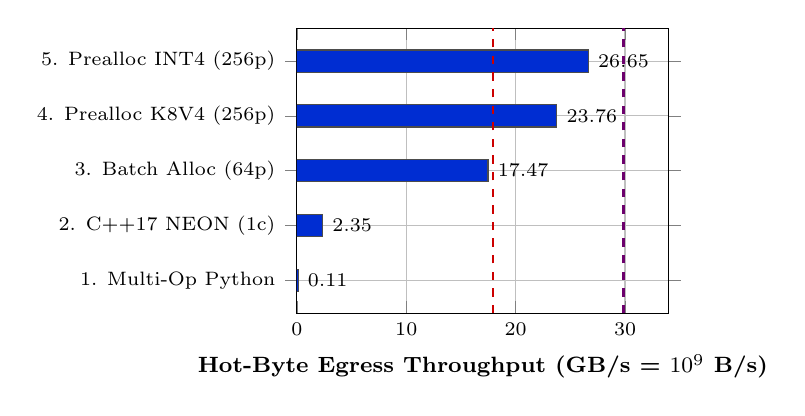
\begin{tikzpicture}
\begin{axis}[
    xbar,
    width=0.52\columnwidth,
    height=5.2cm,
    xmin=0, xmax=34,
    ymin=0.4, ymax=5.6,
    xlabel={Hot-Byte Egress Throughput (GB/s = $10^9$ B/s)},
    ytick={1,2,3,4,5},
    yticklabels={
        {1. Multi-Op Python},
        {2. C++17 NEON (1c)},
        {3. Batch Alloc (64p)},
        {4. Prealloc K8V4 (256p)},
        {5. Prealloc INT4 (256p)}
    },
    nodes near coords,
    nodes near coords align={horizontal},
    every node near coord/.append style={font=\scriptsize\bfseries},
    bar width=8pt,
    grid=major,
    tick label style={font=\scriptsize},
    label style={font=\footnotesize\bfseries}
]
\addplot[fill=blue!65!teal, draw=black!70] coordinates {
    (0.11,1)
    (2.35,2)
    (17.47,3)
    (23.76,4)
    (26.65,5)
};
\draw[red!80!black, thick, dashed] (axis cs:17.93,0.4) -- (axis cs:17.93,5.6);
\draw[violet!85!black, thick, dashed] (axis cs:29.85,0.4) -- (axis cs:29.85,5.6);
\end{axis}
\end{tikzpicture}
\caption{Measured cold-page egress throughput tiers on Apple M3 Max ($N=5$ independent process runs). Dashed lines denote the 100GbE RoCEv2 Theorem~1 break-even threshold (17.93 GB/s hot, red) and 100GbE full wire-saturation threshold (29.85 GB/s hot, violet).}
\label{fig:throughput}
\end{figure}

\begin{table}[htbp]
\centering
\caption{Measured Kernel Latency \& Throughput on 262,144 B (256 KiB) GQA Page ($N=5$ Independent Process Runs $\times 50$ Iterations; RFC 8439 ChaCha20 + SipHash-2-4-128 in Tiers 2--5).}
\label{tab:kernel_progression}
\resizebox{\columnwidth}{!}{
\begin{tabular}{lrrrrrr}
\toprule
\textbf{Measured Implementation Tier} & \textbf{Egress ($\mu$s/p)} & \textbf{Ingress ($\mu$s/p)} & \textbf{Hot (GB/s)} & \textbf{Wire (GB/s)} & \textbf{vs.\ Py} & \textbf{vs.\ 1c} \\
\midrule
1. Multi-Op Python (1c, BLAKE2b) & 2,322.4 $\pm$ 36.2 & 1,838.3 $\pm$ 40.8 & 0.11 $\pm$ 0.00 & 0.04 $\pm$ 0.00 & 1.0$\times$ & 0.05$\times$ \\
2. C++17 NEON (1c, INT4) & 111.4 $\pm$ 0.6 & 113.1 $\pm$ 0.4 & 2.35 $\pm$ 0.01 & 0.88 $\pm$ 0.01 & 20.9$\times$ & 1.00$\times$ \\
3. Batch w/ Alloc (64p, INT4) & 15.02 $\pm$ 0.38 & 11.39 $\pm$ 0.19 & 17.47 $\pm$ 0.43 & 6.55 $\pm$ 0.16 & 154.8$\times$ & 7.42$\times$ \\
4. Peak Prealloc CPU (256p, K8V4) & 11.04 $\pm$ 0.13 & --- & 23.76 $\pm$ 0.27 & 10.40 $\pm$ 0.12 & 210.4$\times$ & 10.09$\times$ \\
\textbf{5. Peak Prealloc CPU (256p, INT4)} & \textbf{9.84 $\pm$ 0.17} & \textbf{10.15 $\pm$ 0.11} & \textbf{26.65 $\pm$ 0.46} & \textbf{10.00 $\pm$ 0.17} & \textbf{236.1$\times$} & \textbf{11.32$\times$} \\
\bottomrule
\end{tabular}
}
\end{table}

\textbf{Incremental Implementation-Tier Comparisons (Not Controlled Causal Ablations):} The cumulative \textbf{236.05 $\pm$ 4.76$\times$} ratio over Tier~1 and the intermediate step ratios in Table~\ref{tab:kernel_progression} are \textit{incremental implementation-tier comparisons across compounded system changes}, not controlled single-factor causal ablations isolating register fusion alone: (1) moving from Tier~1 to Tier~2 (\textbf{20.85 $\pm$ 0.29$\times$}) simultaneously replaces multi-operator Python/PyTorch and \texttt{BLAKE2b-128} with compiled C++17 (\texttt{-O3 -march=armv8.5-a+fp16}), \texttt{FP32}-reciprocal-narrowed-to-\texttt{FP16} NEON quantization, 4-block vectorized ChaCha20, \texttt{SipHash-2-4-128}, and in-register vector encryption/MAC absorption (with L1 stack scale staging); (2) moving from Tier~2 to Tier~3 (\textbf{7.42 $\pm$ 0.20$\times$} over 1-core C++) parallelizes a 64-page batch via Grand Central Dispatch (\texttt{dispatch\_apply\_f}) including per-call output tensor allocation and keyring nonce reservation (\textbf{17.47 $\pm$ 0.43 GB/s} hot egress and \textbf{23.02 $\pm$ 0.38 GB/s} hot ingress); and (3) moving from Tier~3 to Tier~5 (\textbf{1.53$\times$} over Tier~3, \textbf{11.32 $\pm$ 0.23$\times$} over 1-core C++) simultaneously increases the batch size from 64 to 256 pages and writes into a \textbf{caller-preallocated CPU \texttt{uint8} tensor buffer} (avoiding per-call output allocation in the loop, without performing hardware RDMA NIC memory registration), reaching \textbf{26.65 $\pm$ 0.46 GB/s} hot egress (median \textbf{26.67 GB/s}, range $26.00$--$27.09\text{ GB/s}$) and \textbf{25.84 $\pm$ 0.28 GB/s} hot ingress.

\subsection{Analytical Serial-Egress RDMA Transfer Latency Model}
Table~\ref{tab:rdma_transfer} evaluates an \textbf{analytical serial-egress model} ($T_{\text{total}} = T_{\text{compute}} + T_{\text{wire}}$, not a live NIC-to-NIC RDMA measurement) for offloading a 4,096-token prefix across 64 layers ($4,096\text{ pages} = 1,073.74\text{ MB}$ SI / $1,024.0\text{ MiB}$ raw \texttt{BF16}) at an assumed 100GbE RoCEv2 goodput of $BW_{\text{net}} = 11.2\text{ GB/s}$ ($11.2 \times 10^9\text{ B/s}$). We explicitly separate \textbf{analytical latency using empirically measured Apple M3 Max CPU fused compute} (Rows 4a and 5a) from the \textbf{hypothetical GPU SRAM ($950\text{ GB/s}$) analytical projection} (Rows 4b and 5b). Combining measured CPU compute ($40.31 \pm 0.70\text{ ms}$) with analytical 100GbE wire transfer ($35.97\text{ ms}$), serial ZTCP \texttt{INT4} achieves \textbf{76.28 $\pm$ 0.70 ms} vs.\ \textbf{95.87 ms} for unencrypted raw \texttt{BF16} (\textbf{1.26 $\pm$ 0.01$\times$} speedup, consistent across both the ratio of 5-run mean latencies $95.87 / 76.28 = 1.2568\times$ and the mean of 2-decimal rounded per-run ratios $[1.25, 1.27, 1.27, 1.24, 1.26]$ in \texttt{latest\_results.json}), while \texttt{K8V4} achieves \textbf{87.15 $\pm$ 0.53 ms} (\textbf{1.10 $\pm$ 0.01$\times$} speedup).

\begin{table}[htbp]
\centering
\caption{Analytical Serial-Egress 4,096-Token Prefix Transfer Model across 64 Layers ($11.2\text{ GB/s}$ SI Goodput), Separating Measured M3 Max CPU Compute from Projected GPU SRAM ($950\text{ GB/s}$).}
\label{tab:rdma_transfer}
\resizebox{\columnwidth}{!}{
\begin{tabular}{lrrrrr}
\toprule
\textbf{Analytical Serial Pipeline Path} & \textbf{Wire (MB / MiB)} & \textbf{Compute} & \textbf{Wire} & \textbf{Total} & \textbf{Speedup} \\
\midrule
1. Unencrypted Raw BF16 Baseline & 1,073.7 / 1,024.0 & 0.00 ms & 95.87 ms & 95.87 ms & 1.00$\times$ \\
2. Discrete Host Copy (28 GB/s) + K8V4 & 470.0 / 448.2 & 38.35 ms & 41.96 ms & 80.31 ms & 1.19$\times$ \\
3. Unencrypted Raw FP8 (Hot Quant.) & 536.9 / 512.0 & 0.00 ms & 47.93 ms & 47.93 ms & 2.00$\times$ \\
\textbf{4a. ZTCP K8V4 (Measured M3 Max CPU)} & \textbf{470.0 / 448.2} & \textbf{45.19 ms} & \textbf{41.96 ms} & \textbf{87.15 ms} & \textbf{1.10$\times$} \\
\textbf{5a. ZTCP INT4 (Measured M3 Max CPU)} & \textbf{402.8 / 384.2} & \textbf{40.31 ms} & \textbf{35.97 ms} & \textbf{76.28 ms} & \textbf{1.26$\times$} \\
4b. ZTCP K8V4 (Projected GPU @ 950 GB/s) & 470.0 / 448.2 & 1.13 ms & 41.96 ms & 43.09 ms & 2.22$\times$ \\
5b. ZTCP INT4 (Projected GPU @ 950 GB/s) & 402.8 / 384.2 & 1.13 ms & 35.97 ms & 37.10 ms & 2.58$\times$ \\
\bottomrule
\end{tabular}
}
\end{table}

\subsection{Security Verification Matrix, Protocol Contracts \& Limitations}
Table~\ref{tab:security_matrix} summarizes the automated security verification suite bundled in \texttt{bench\_cold\_page\_pipeline.py} (\texttt{run\_security\_verification}), specifying the exact exercised backend for each test group and labeling local in-memory byte/bit mutations as simulated RDMA tampering. (In-flight egress and ingress shred checks across all four codec paths \texttt{py\_single}, \texttt{cpp\_single}, \texttt{cpp\_batch}, and \texttt{cpp\_peak} are verified in the separate local regression suite \texttt{verify\_package2.py}, section \texttt{CODE-003}; overlapping-batch nonce checks are verified in section \texttt{B6-2}, distinct from the bundled benchmark.)

\begin{table}[htbp]
\centering
\caption{Bundled Security, Freshness \& Concurrency Matrix by Backend (\texttt{bench\_cold\_page\_pipeline.py}).}
\label{tab:security_matrix}
\resizebox{\columnwidth}{!}{
\begin{tabular}{lllll}
\toprule
\textbf{Test ID} & \textbf{Backend Path} & \textbf{Verified Scenario} & \textbf{Observed Outcome} & \textbf{Status} \\
\midrule
3.1--3.4 & Py Ref (\texttt{BLAKE2b}) & Round-Trip, AAD, Sim.\ 1b Flip, Shred & \texttt{CrossTenant} / \texttt{KVIntegrityError} & \textbf{PASS} \\
3.5 & C++ Peak (\texttt{SipHash}) & Native Peak Decode \& Cache Re-Read & Exact Decode ($\times 2$) & \textbf{PASS} \\
3.6--3.8 & C++ Peak (\texttt{SipHash}) & Sim.\ Scale, 16B Swap \& V Bit Tamper & \texttt{KVIntegrityError} & \textbf{PASS} \\
3.9, 3.11 & C++ Peak (\texttt{SipHash}) & 4$\times$ AAD Drift \& Post-Shred Re-Derive & \texttt{CrossTenant} / \texttt{KVIntegrityError} & \textbf{PASS} \\
3.10a--c & C++ Peak + Py Nonce & Nonce Helper, Peak Dup Nonce \& Stale Replay & \texttt{NonceReuse} / \texttt{StalePageReplay} & \textbf{PASS} \\
3.12 & C++ Peak \& Single & Peak Same-Nonce Race; 1p Burn \& Watermark & \texttt{NonceReuse} / \texttt{StalePageReplay} & \textbf{PASS} \\
\bottomrule
\end{tabular}
}
\end{table}

\textbf{Implementation Scope, Protocol Contracts \& Open Caveats:}
\begin{enumerate}
    \item \textbf{In-Process Keyring Concurrency, Linearization \& Buffer Ownership Contracts (\texttt{CODE-003}):}
    (a) \textit{Single-process lock scope:} Thread safety, atomic nonce burning, and monotonic watermarks are enforced in-memory within a single Python process via \texttt{threading.RLock} (verified by bounded multi-threaded tests).
    (b) \textit{Pre-shred linearization:} Operations whose locked \texttt{commit\_egress} or \texttt{finish\_ingress} check completes \textit{before} \texttt{crypto\_shred\_session} acquires the lock are linearized prior to the shred and may return normally after the concurrent shred call returns; operations reaching \texttt{begin\_egress\_execution}, \texttt{commit\_egress}, or \texttt{finish\_ingress} \textit{after} shred zeroize outputs populated in their execution block (\texttt{out\_blobs\_u8.zero\_()} / \texttt{k\_out.zero\_()}) and raise \texttt{SessionShreddedError}.
    (c) \textit{Peak buffer ownership \& exception invalidation:} The caller of \texttt{encode\_cold\_pages\_peak\_into} (and \texttt{decode\_cold\_pages\_peak\_into}) must exclusively own the preallocated output buffer, read/publish it only after a normal return, and discard it as invalid on \textit{any} exception; preflight errors in \texttt{preflight\_validate\_egress} and input/output buffer-overlap checks occur before the buffer-zeroing \texttt{try...except} block and do not clear prior buffer contents.
    (d) \textit{User-space memory boundary:} While mutable \texttt{bytearray(32)} key buffers and per-call mutable snapshots are wiped in-place, immutable Python \texttt{bytes}, native C++ stack/integer key copies ($k_0..k_3$, $mk_0..mk_1$), CPython GC temporaries, and OS swap/core-dumps remain outside any hardware memory-erasure guarantee.
    \item \textbf{Wire Version, Backend MAC Non-Interoperability, Binding Defaults \& Verified Build Scope:} The 32B header retains \texttt{FORMAT\_VERSION = 1}. The Python reference codec uses 128-bit \texttt{BLAKE2b} whereas the native C++17 codec uses 128-bit \texttt{SipHash-2-4-128}; each backend decodes its own blobs. Low-level pybind11 entrypoints keep default \texttt{k2=0, k3=0} arguments for legacy signature compatibility while \texttt{NativeCppFusedColdPageCodec} always passes all 256 bits ($k_0..k_3$). Finally, \texttt{native\_fused\_codec.py} passes \texttt{-march=armv8.5-a+fp16} unconditionally on POSIX builds (verified on Apple Silicon \texttt{arm64}), and \texttt{--reaggregate-only} updates its target JSON file in place unless \texttt{--output-json} is directed to a scratch copy.
\end{enumerate}

\section{Conclusion \& Artifact Availability}
ZTCP demonstrates that confidential KV-cache offloading over RDMA can achieve net latency reductions over unencrypted raw transfers whenever fused throughput exceeds the Theorem~1 break-even bound. By combining RoPE-preserving asymmetric quantization with 256-bit RFC 8439 ChaCha20 encryption, 128-bit SipHash-2-4-128 authentication, and transactional session-state management, ZTCP shrinks cold-page wire footprints by $2.67\times$--$2.94\times$, reaches $26.65 \pm 0.46\text{ GB/s}$ hot ($10.00 \pm 0.17\text{ GB/s}$ wire) egress and $25.84 \pm 0.28\text{ GB/s}$ hot ingress throughput on an Apple M3 Max CPU ($1.26 \pm 0.01\times$ faster in our analytical serial-egress 100GbE model using measured CPU compute time, and $2.22\times$--$2.58\times$ under projected GPU SRAM execution), and enforces verifiable multi-tenant isolation, freshness, and in-process crypto-shredding.

\textbf{Code \& Reproducible Benchmarks:} The open-source C++17 ARMv8.5-A FP16 NEON codec, 32-byte AAD wire specification, zero-copy upstream plugin hooks (\texttt{sglang}, \texttt{lmcache}, \texttt{mooncake}), and reproducible 5-run benchmark artifacts are publicly available at \url{https://github.com/Theseus-Guard/ZTCP} and archived under CERN/Zenodo DOI \href{https://doi.org/10.5281/zenodo.23555749}{\texttt{10.5281/zenodo.23555749}}.

\bibliographystyle{plain}
\bibliography{references}

\end{document}
